\documentclass[10pt]{beamer} 
     \hypersetup{pdfpagemode=FullScreen} 
     \usepackage{tikz} 
     \usetikzlibrary{shadows,patterns,shapes} 
     \usetikzlibrary{shapes.arrows,chains} 
     % serifenfreier Font -- fuer Praesentation geeignet/er 
     \listfiles % damit im Log alle benutzten Pakete aufgelistet werden 
     \usetheme[progressbar=frametitle]{metropolis} 
     \usepackage{appendixnumberbeamer} 
     \usepackage{booktabs} 
     \usepackage[scale=2]{ccicons} 
     \usepackage[utf8]{inputenc} 
     \usepackage{pgfplots} 
     \usepgfplotslibrary{dateplot} 
     \usepackage[ngerman]{babel} 
     \usepackage{xspace} 
     \usebackgroundtemplate{
     \tikz[overlay,remember picture] 
     \node[opacity=0.3, at=(current page.south east),anchor=south east,inner sep=0pt] {
     
\includegraphics[width=1.53\textwidth]{./PDFcreater/Pictures/background.png}};
     } 
     %\usebackgroundtemplate{
\includegraphics[,right]{./PDFcreater/Pictures/background.png}}
     \definecolor{Purple}{HTML}{6D087C}
     \definecolor{Orange}{HTML}{CF4A30}
     
     % Theme colors are derived from these two elements
     \setbeamercolor{alerted text}{fg=Orange}
     
     % ... however you can of course override styles of all elements 
     \setbeamercolor{frametitle}{bg=Purple}
     
     \title{Feedback der Studierenden im Kurs: SolidEdge } 
     \begin{document} 
     \maketitle 
\begin{frame}[fragile]{1Geschlecht der Studis} 
 \begin{figure}
 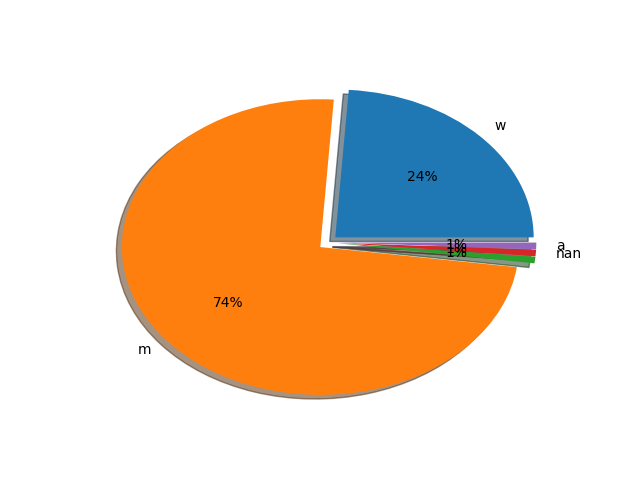
\includegraphics[width= 0.9\linewidth]{./PDFcreater/Plots/SolidEdge/1Geschlecht+der+Studis.png};
 \end{figure}
 \end{frame}
\begin{frame}[fragile]{1Studiengang der Studis} 
 \begin{figure}
 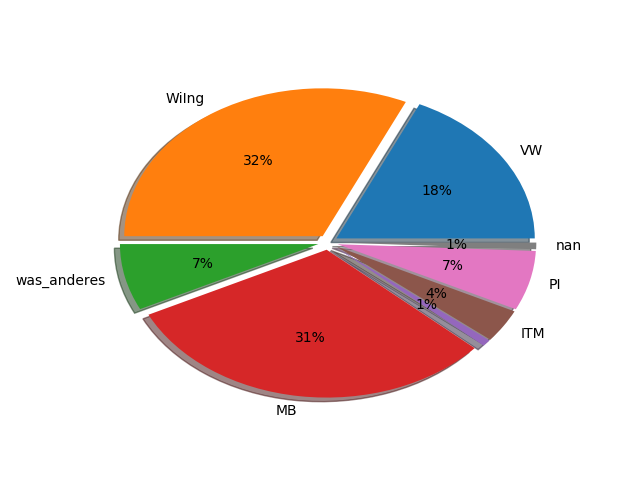
\includegraphics[width= 0.9\linewidth]{./PDFcreater/Plots/SolidEdge/1Studiengang+der+Studis.png};
 \end{figure}
 \end{frame}
\begin{frame}[fragile]{1Tutor der Studis} 
 \begin{figure}
 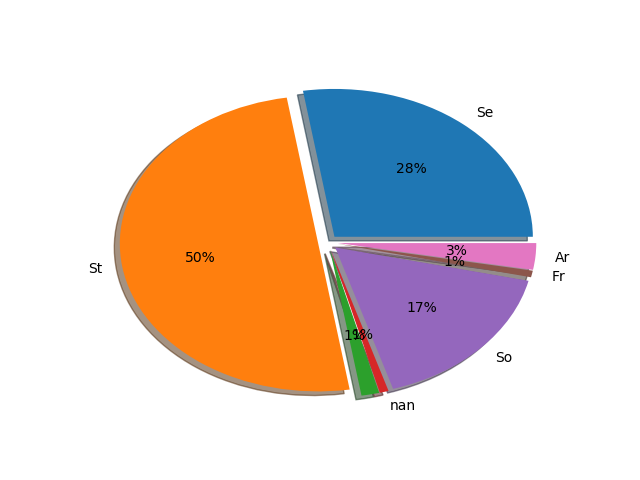
\includegraphics[width= 0.9\linewidth]{./PDFcreater/Plots/SolidEdge/1Tutor+der+Studis.png};
 \end{figure}
 \end{frame}
\begin{frame}[fragile]{Benoetigte Stundenzahl vom gesamten CAD Kurs pro Woche} 
 \begin{figure}
 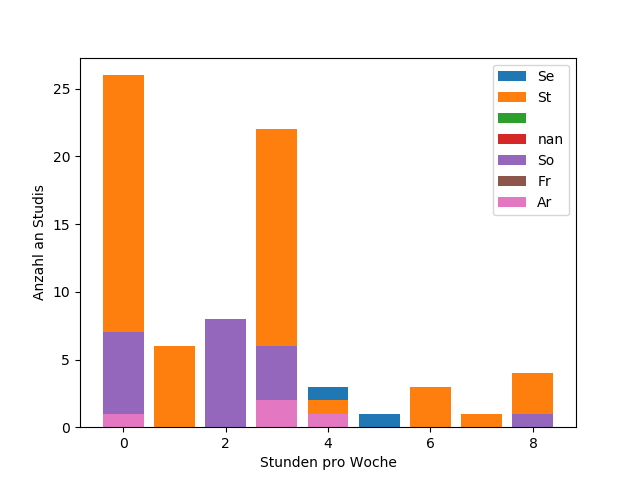
\includegraphics[width= 0.9\linewidth]{./PDFcreater/Plots/SolidEdge/Benoetigte+Stundenzahl+vom+gesamten+CAD+Kurs+pro+Woche.png};
 \end{figure}
 \end{frame}
\begin{frame}[fragile]{Der Lehrinhalt war ausreichend um die HA zu bearbeiten} 
 \begin{figure}
 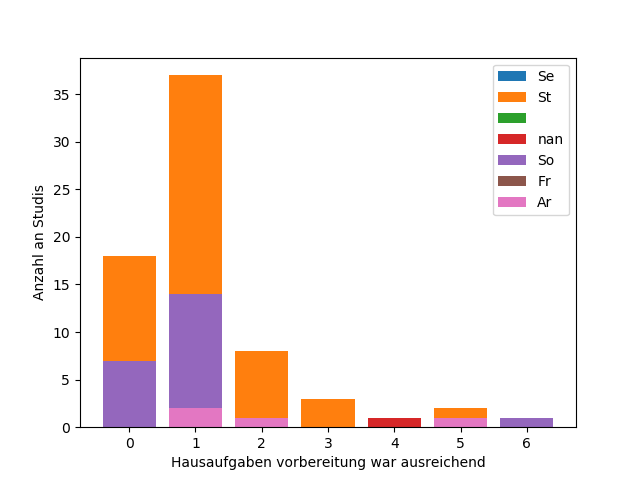
\includegraphics[width= 0.9\linewidth]{./PDFcreater/Plots/SolidEdge/Der+Lehrinhalt+war+ausreichend+um+die+HA+zu+bearbeiten.png};
 \end{figure}
 \end{frame}
\begin{frame}[fragile]{Der Schwierigkeitsgrad war hoch} 
 \begin{figure}
 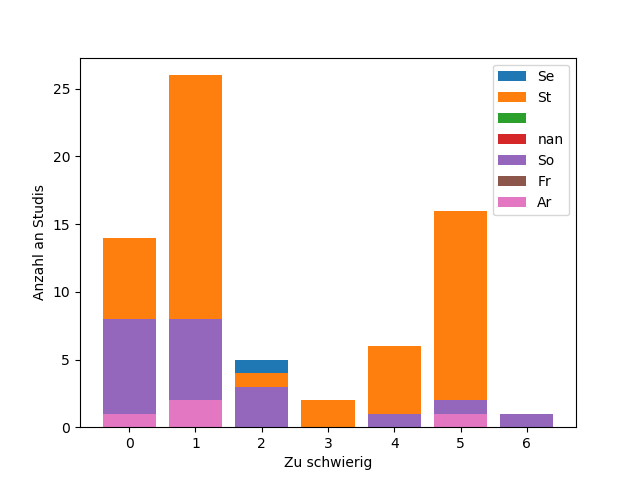
\includegraphics[width= 0.9\linewidth]{./PDFcreater/Plots/SolidEdge/Der+Schwierigkeitsgrad+war+hoch.png};
 \end{figure}
 \end{frame}
\begin{frame}[fragile]{Die Formulierungen in der Hausaufgabe waren eindeutig} 
 \begin{figure}
 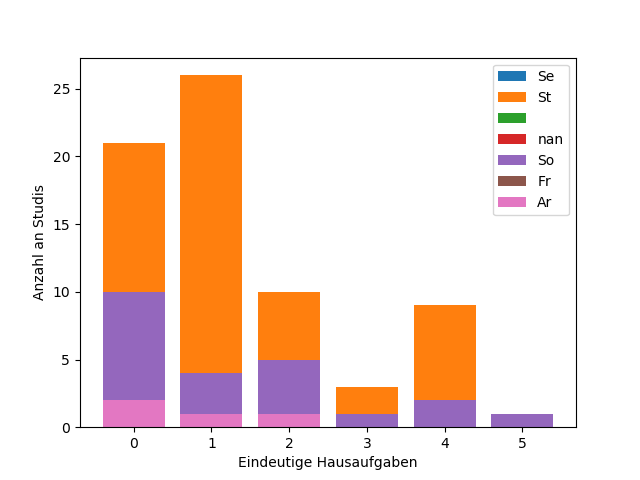
\includegraphics[width= 0.9\linewidth]{./PDFcreater/Plots/SolidEdge/Die+Formulierungen+in+der+Hausaufgabe+waren+eindeutig.png};
 \end{figure}
 \end{frame}
\begin{frame}[fragile]{Die Hausaufgabe sollte vom Umfang her reduziert werden} 
 \begin{figure}
 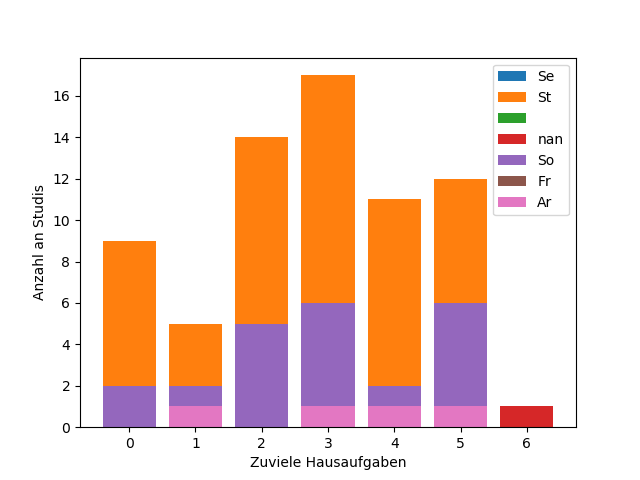
\includegraphics[width= 0.9\linewidth]{./PDFcreater/Plots/SolidEdge/Die+Hausaufgabe+sollte+vom+Umfang+her+reduziert+werden.png};
 \end{figure}
 \end{frame}
\begin{frame}[fragile]{Die Uebungen sind gut strukturiert} 
 \begin{figure}
 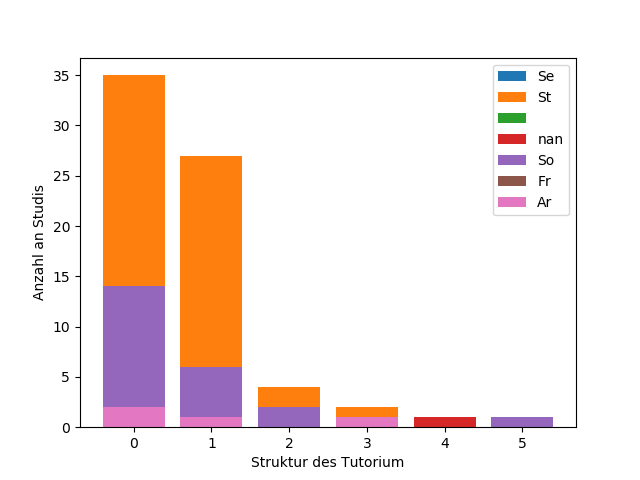
\includegraphics[width= 0.9\linewidth]{./PDFcreater/Plots/SolidEdge/Die+Uebungen+sind+gut+strukturiert.png};
 \end{figure}
 \end{frame}
\begin{frame}[fragile]{Die Uebungsbeispiele sind gut gewaehlt} 
 \begin{figure}
 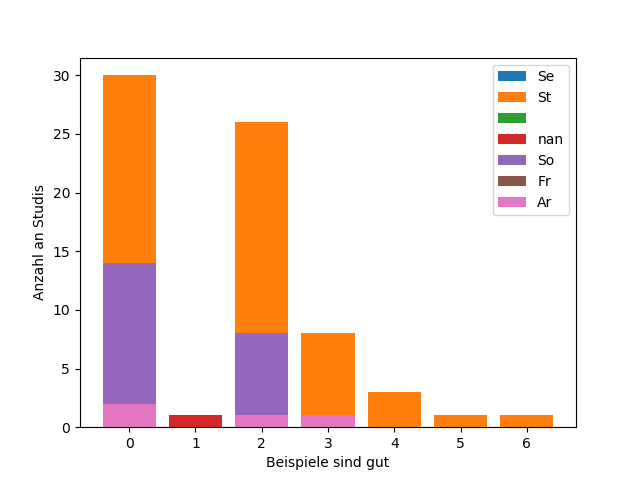
\includegraphics[width= 0.9\linewidth]{./PDFcreater/Plots/SolidEdge/Die+Uebungsbeispiele+sind+gut+gewaehlt.png};
 \end{figure}
 \end{frame}
\begin{frame}[fragile]{Ich habe die Uebungsaufgaben alle gemacht} 
 \begin{figure}
 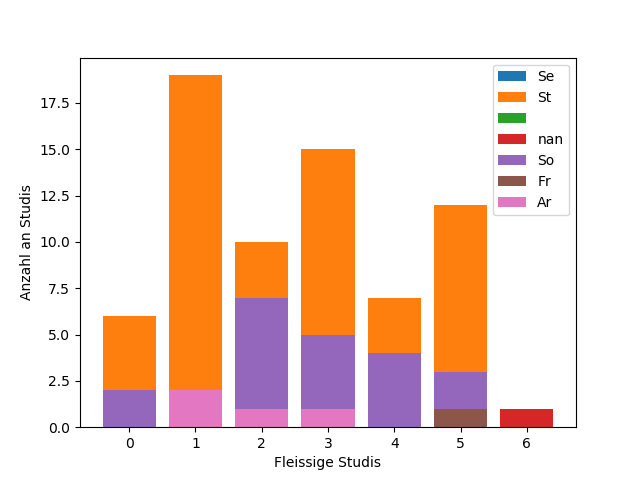
\includegraphics[width= 0.9\linewidth]{./PDFcreater/Plots/SolidEdge/Ich+habe+die+Uebungsaufgaben+alle+gemacht.png};
 \end{figure}
 \end{frame}
\begin{frame}[fragile]{Ich habe mich schon fruehzeitig mit dem Programm zu Hause beschaeftigt} 
 \begin{figure}
 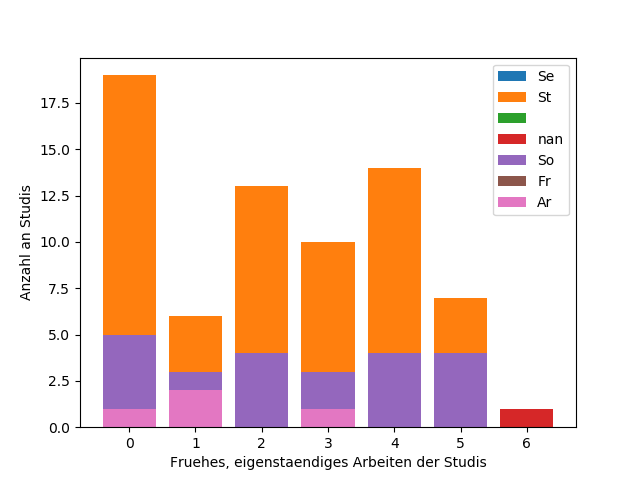
\includegraphics[width= 0.9\linewidth]{./PDFcreater/Plots/SolidEdge/Ich+habe+mich+schon+fruehzeitig+mit+dem+Programm+zu+Hause+beschaeftigt.png};
 \end{figure}
 \end{frame}
\begin{frame}[fragile]{Ich habe viel Zeit zur Bearbeitung der Hausaufgabe benoetigt} 
 \begin{figure}
 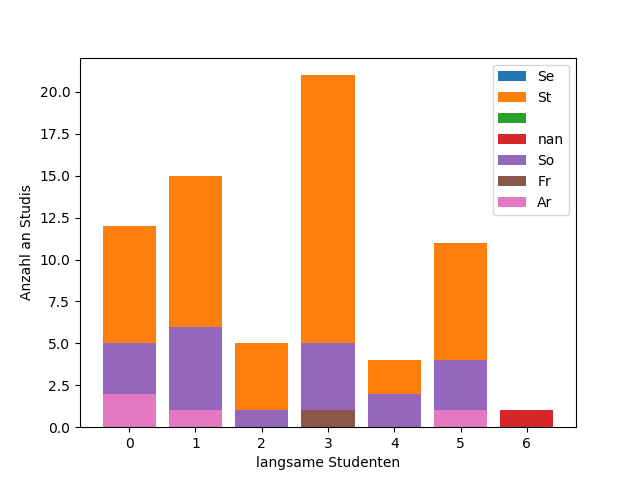
\includegraphics[width= 0.9\linewidth]{./PDFcreater/Plots/SolidEdge/Ich+habe+viel+Zeit+zur+Bearbeitung+der+Hausaufgabe+benoetigt.png};
 \end{figure}
 \end{frame}
\begin{frame}[fragile]{Ich haette gerne mehr Uebungsaufgaben gehabt} 
 \begin{figure}
 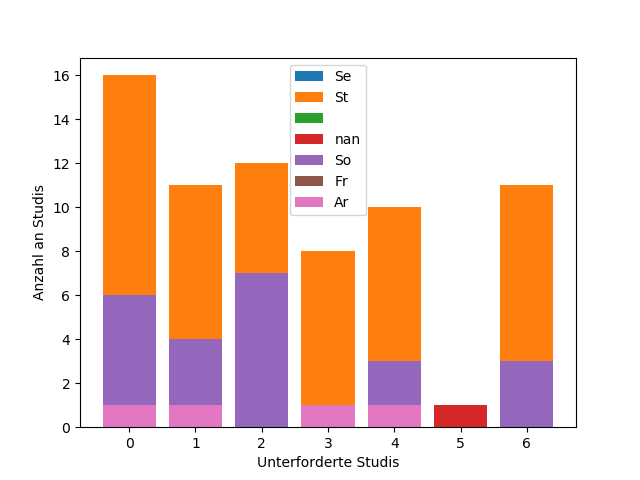
\includegraphics[width= 0.9\linewidth]{./PDFcreater/Plots/SolidEdge/Ich+haette+gerne+mehr+Uebungsaufgaben+gehabt.png};
 \end{figure}
 \end{frame}
\begin{frame}[fragile]{Ich war immer gut auf das Tutorium vorbereitet} 
 \begin{figure}
 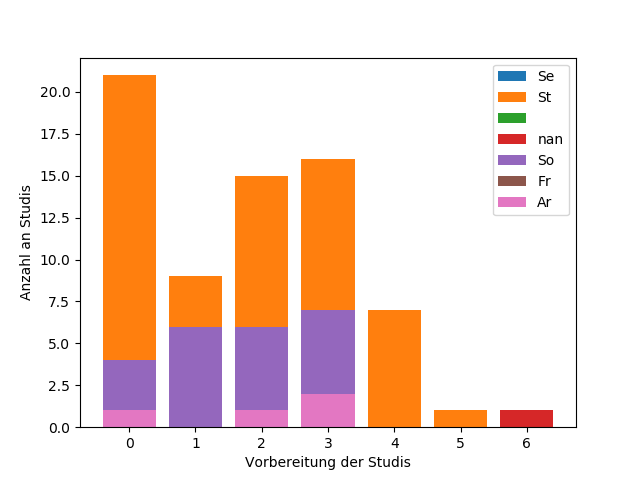
\includegraphics[width= 0.9\linewidth]{./PDFcreater/Plots/SolidEdge/Ich+war+immer+gut+auf+das+Tutorium+vorbereitet.png};
 \end{figure}
 \end{frame}
\begin{frame}[fragile]{Semester der Studierenden} 
 \begin{figure}
 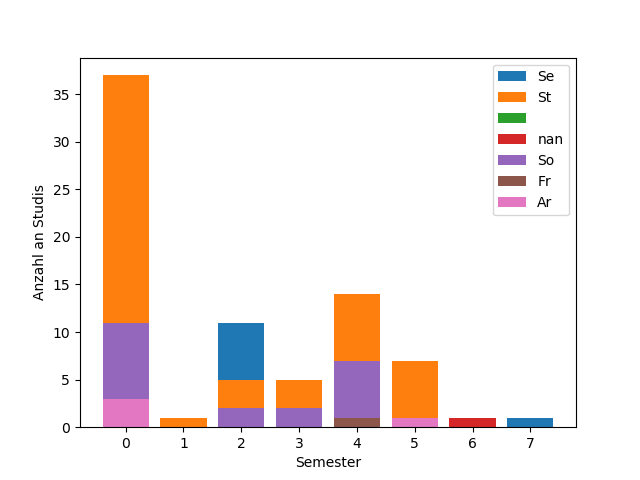
\includegraphics[width= 0.9\linewidth]{./PDFcreater/Plots/SolidEdge/Semester+der+Studierenden.png};
 \end{figure}
 \end{frame}
\begin{frame}[fragile]{Tutor foerdert aktive Teilnahme der Studenten} 
 \begin{figure}
 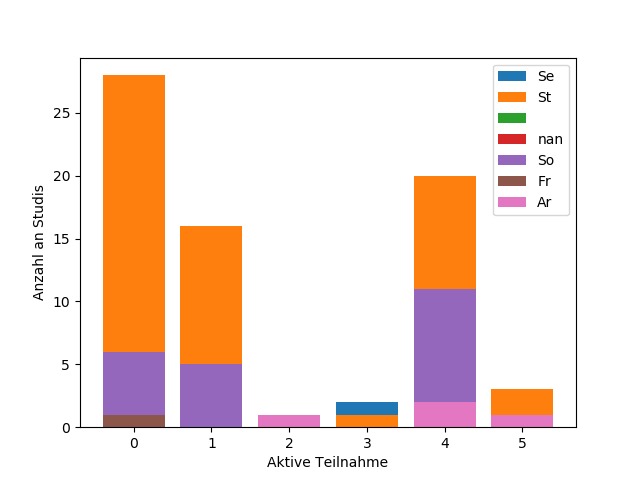
\includegraphics[width= 0.9\linewidth]{./PDFcreater/Plots/SolidEdge/Tutor+foerdert+aktive+Teilnahme+der+Studenten.png};
 \end{figure}
 \end{frame}
\begin{frame}[fragile]{Tutor ist immer gut auf das Tutorium vorbereitet} 
 \begin{figure}
 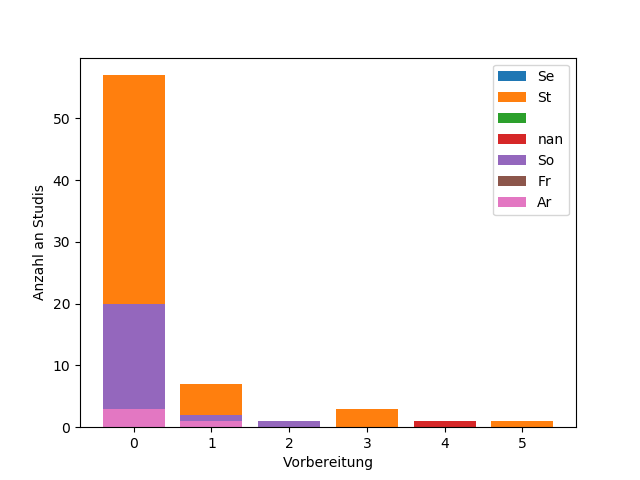
\includegraphics[width= 0.9\linewidth]{./PDFcreater/Plots/SolidEdge/Tutor+ist+immer+gut+auf+das+Tutorium+vorbereitet.png};
 \end{figure}
 \end{frame}
\begin{frame}[fragile]{Tutor kann den Lehrinhalt verstaendlich darlegen} 
 \begin{figure}
 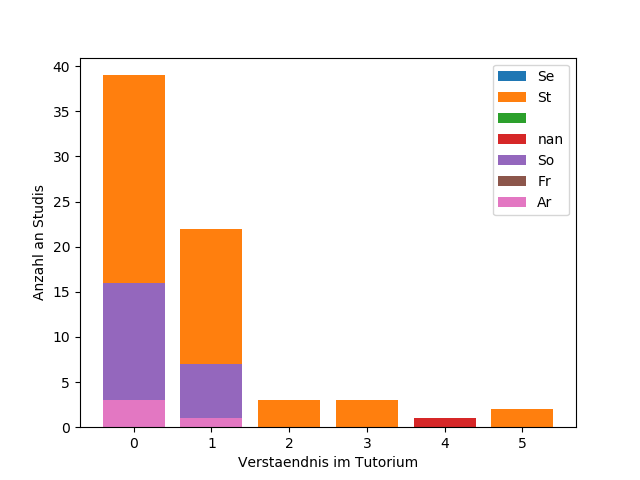
\includegraphics[width= 0.9\linewidth]{./PDFcreater/Plots/SolidEdge/Tutor+kann+den+Lehrinhalt+verstaendlich+darlegen.png};
 \end{figure}
 \end{frame}
\begin{frame}[fragile]{Kommmentare der Studenten, Tutor: Se}mehr zeit im tut für die übungen zum selber machen, manchmal kam man nicht hinterher;
 \end{frame}
\begin{frame}[fragile]{Kommmentare der Studenten, Tutor: Se} Ich war mit dem Lernergebnis sehr zufrieden.   Bei Verlust des Anschlusses war es in der Übung teils schwierig ihn wieder zu finden.;
 \end{frame}
\begin{frame}[fragile]{Kommmentare der Studenten, Tutor: Se}Gelungen war die Unterrichtsgestaltung sowie die Unterrichtsführung. Etwas negatives fällt mir nicht ein.;
 \end{frame}
\begin{frame}[fragile]{Kommmentare der Studenten, Tutor: Se}man könnte öfter fragen ob alle mitgekommen sind bzw. wo probleme sind    öfter bei den studenten gucken wie die es hinbekommen.;
 \end{frame}
\begin{frame}[fragile]{Kommmentare der Studenten, Tutor: St}Gucken, dass im Tutorium alle bei den Übungsaufgaben mitkommen und helfen, falls einer irgendwo rausfällt.;
 \end{frame}
\begin{frame}[fragile]{Kommmentare der Studenten, Tutor: St}Wenn man interessiert ist, hilft der Tutor sehr gerne auch umfangreich weiter. Außerdem gibt er gute Tipps und kennt SE in und auswendig. Manchmal hat man den Anschluss verloren, weil man eine Funktion nicht sofort gefunden hat, ab und zu wäre die Frage: "Sind alle mitgekommen?" angemessen, um wieder einsteigen zu können.
 Sonst ein sehr guter strukturierter SE Kurs;
 \end{frame}
\begin{frame}[fragile]{Kommmentare der Studenten, Tutor: St}Zu Beginn des Semesters wurde das Skizzieren in den Tutorien sehr ausführlich behandelt; im weiteren Verlauf wurden wesentlich kompliziertere Arbeitsschritte und Anwendungen (z.B. die drei Möglichkeiten zum Erstellen von Ausbrüchen, Zeichnungsableitung) in einem höheren Tempo erklärt und abgearbeitet. Mir hätte es geholfen, die Übungen zum Skizzieren früher abzuschließen und dafür mehr Zeit für nachfolgende Themen zu verwenden.;
 \end{frame}
\begin{frame}[fragile]{Kommmentare der Studenten, Tutor: St}Ich fande es sehr interessant, dass wir am letzten Tutoriumstermin Einblicke in die Geschichte der TU und den Unfall des Space Shuttles bekommen haben.;
 \end{frame}
\begin{frame}[fragile]{Kommmentare der Studenten, Tutor: St}Ich finde es wunderbar, dass die Tutoren sehr kompetent und immer bereit sind, den Studierenden bei Kursschwierigkeiten zu helfen. Emails wurden auch sehr schnell beantwortet, sodass man an den CAD Übungen und der Hausaufgabe auch zuhause weiter arbeiten konnte.;
 \end{frame}
\begin{frame}[fragile]{Kommmentare der Studenten, Tutor: Se}Besseres Begleitmaterial   > Folien waren ganz gut, jedoch nur für die Grundlagen, Anleitungen für Zusammenbau etc. wäre ganz gut ;
 \end{frame}
\begin{frame}[fragile]{Kommmentare der Studenten, Tutor: St}Stefan hat stets ein sehr gutes Tutorium gehalten. Manchmal war das Tempo etwas zu hoch. Wenn man sich halbwegs angestrengt, ist es angenehm, mitzukommen. Er bringt viel Fachwissen rüber und vermittelt einen sehr kompetenten Eindruck. Ich würde mich freuen, wenn die Tutoren in den Sprechstunden rumgehen würden und maximal eine Frage pro Student auf einmal beanworten, wenn die Sprechstunde voll ist.;
 \end{frame}
\begin{frame}[fragile]{Kommmentare der Studenten, Tutor: Se}Am Anfang sollte gesagt werden, dass es so gedacht ist, dass man die Hausaufgabe parallel zum Kurs bearbeitet. Ich dachte das wäre erst fürs Ende des Kurses vorgesehen und wusste auch nicht, dass es so eine ausführliche Anleitung gibt und habe mir die HA daher erst angeguckt, als auf Isis geschrieben wurde, dass man die Welle abgeben soll. ;
 \end{frame}
\begin{frame}[fragile]{Kommmentare der Studenten, Tutor: St}   mir war zu Anfang(vor dem ersten CAD Tutorium) nicht bewusst, dass das Tutorium "nur" eine Stunde lang ist, könnte man z.B. in der erste K1 VL ansagen, wegen besserer Zeitplanung/Stundenplangestaltung     die Tutoren sind freundlich   auch nach Tutorium Hilfe   es wurde auch über den Telleradn hinaus geschaut (z.B. Feingewinde erklärt etc.)   letzte Tutorien Woche: Vortrag zu historischen Ereignissen im Ingenieruswesen war sehr lehrreich und hat zum nachdenken angeregt;
 \end{frame}
\begin{frame}[fragile]{Kommmentare der Studenten, Tutor: St}Zum Teil etwas zu schnell. Oft konnte ich nicht bei allen Schritten folgen und mitmachen, sodass einige Schritte nicht klar geworden sind und doch einiges beim selstständigen Baerbeiten ausprobiert werden muste. Etwas mehr selbständiges Arbeiten, wobei der Tutor herumgehen und Fragen beantworten sollte. Insegsamt ein sehr lehrreiches Modul. Die Hausuafgabe eignet sich sehr gut zum Erlernen und Vertiefen der Modulinhalte. Sehr genaue Aufgabenstellung, die sich gut bearbeiten lässt.;
 \end{frame}
\begin{frame}[fragile]{Kommmentare der Studenten, Tutor: St}Verbesserungswürdig: Es war oft schwierig, bei dem Bearbeitungstempo im Tutorium jeden Schritt nachzuvollziehen, geschweige denn umzusetzen. So kann es schnell dazu kommen, dass man nicht mehr mitkommt und die Motivation für den Rest der Stunde rapide nachlässt.
 
 Gut: Hausaufgaben PDF war zwar sehr umfangreich, dafür war jeder Schritt detailliert beschrieben, sodass man nicht auf perfekte Methodenkenntnis aus dem Tutorium angewiesen war.;
 \end{frame}
\begin{frame}[fragile]{Kommmentare der Studenten, Tutor: St}Tutoriumszeit verlängern. Wenn man nämlich erst einmal beim Stoff zurückfällt, ist es schwer wieder auf den Stand des Tutors zu kommen. Dies führt schnell zu Frustration. D.h. das Tutorium ist etwas zu schnell.;
 \end{frame}
\begin{frame}[fragile]{Kommmentare der Studenten, Tutor: Se}Ich finde gut, dass es Video Tutorials gibt. Sie könnten jedoch besser gestaltet sein, dh. mit Ton für Erklärungen statt mit reinen Texten im Film. Die Hausaufgabe war eine gute Vorbereitung für die letzte Hausaufgabe in K1.;
 \end{frame}
\begin{frame}[fragile]{Kommmentare der Studenten, Tutor: St}Ich fand die Vorführung bevor die Übungsaufgaben bearbeitet wurden gut, jedoch würde es mir lieber sein, wenn man nicht jeden Schritt für verständlich hält und nicht z.B. 3 Schritte nacheinander schnell eingibt und man somit nicht mitbekommen hat, sodass man nicht mehr mitmachen kann, also quasi nur noch bei der Vorführung zuschaut und versucht alle Schritte zu merken.;
 \end{frame}
\begin{frame}[fragile]{Kommmentare der Studenten, Tutor: St}Es war lehrreich nur wenn man einen Moment mal eine Schaltfläche gesucht hat war man hinter her. Das Tempo ist immer sehr rasant. meistens habe ich einfach nur zugehört um möglichst alles mitnehmen zu können. jedoch fehlte mir dann die direkte Anwendung und hatte vergessen wo das Werkzeug zu finden ist.
 Am Ende habe ich aber alles super geschafft. Und selten eine Sprechstunde besucht.
 ;
 \end{frame}
\begin{frame}[fragile]{Kommmentare der Studenten, Tutor: St}Die Übungen sind vom Inhalt her gut und klar strukturiert. Allerdings führt das zügige Tempo dazu, dass man zwar folgen kann, im Nachhinein jedoch nur zum Teil selbstständig die gezeigten Schritte wiederholen kann. Dies mag zum einem dem Umfang des Stoffes geschuldet sein. Ein iterativer Ablauf würde aber sicherlich mehr zum Verständnis beitragen, als erst den Vortrag zu hören und anaschließend Übungen zu bearbeiten.;
 \end{frame}
\begin{frame}[fragile]{Kommmentare der Studenten, Tutor: St}Ich fand es sehr gut wie alles in der Hausaufgabe erklärt wurde. Die Tutorien wären vielleicht ein bisschen besser wenn die Tutoren die Schritte ein bisschen mehr wiederholen würden. Wenn man einen kleinen Schritt verpasst, hat man danach keine Ahnung worum es im Tutorium geht.;
 \end{frame}
\begin{frame}[fragile]{Kommmentare der Studenten, Tutor: St}Kurse 90 minütig gestalten, so dass man das gesamte Wissen über Solid Edge frühzeitig hat um die 4. HA in K1 einfacher zu bewältigen.  ;
 \end{frame}
\begin{frame}[fragile]{Kommmentare der Studenten, Tutor: St}Selber Aufwand wie die K1 4. HA. Warum kann man diese beiden HAs nicht verbinden? Man macht genau dasselbe. Unnötiger hoher Aufwand. Ingesamt in Verbindung zu K1 ein zu hoher Aufwand. Ein Zusatzkurs der circa 3 Stunden die Woche einnimmt und keinen einzigen Leistungspunkt liefert. DAS finde ich mehr als fragwürdig.  In den Tutorien wurde mir persönlich einiges ein wenig zu schnell gemacht, sodass man die Inhalte nicht immer mitbekommen hat, bzw. einige Teilschritte. Zum Glück wurde in der Hausaufgabe (fast) alles gut beschrieben. Leider hing ich trotzdem an zwei bis drei Sachen. Wo ich dafür schnell Hilfe erreiche, war mir nicht so gajnz klar(außer in den CAD Pool zu kommen, was nicht immer eine Möglichkeit ist). Solid Edge auf dem eigenen PC zu nutzen ist eine Katastrophe. Das Programm nahm immer wieder Beziehungen nicht an, die davor genau so funktioniert hatten(Immer aufgeschrieben damit man nicht solange probieren muss, hat am Ende leider nur nichts gebracht). Insgesamt wäre es sinnvoller die Hausaufgabe mehr in die schon sehr überdimensionale Lehrveranstaltung von Konstruktion 1 einzubinden;
 \end{frame}
\begin{frame}[fragile]{Kommmentare der Studenten, Tutor: So}Die Folien bei ISIS hochladen.(letzte tutorien);
 \end{frame}
\begin{frame}[fragile]{Kommmentare der Studenten, Tutor: So}Ich finde eine Stunde ist zu kurz.;
 \end{frame}
\begin{frame}[fragile]{Kommmentare der Studenten, Tutor: So}War eig. allesok, so wie es war!
 Weiter so!;
 \end{frame}
\begin{frame}[fragile]{Kommmentare der Studenten, Tutor: So}Die Gruppen sind etwas groß weshalb auf individuelle Fragen im Tutorium kaum eingegangen werden kann. Ansonsten sehr gute Vorbereitung und Einführung in Solid Edge!;
 \end{frame}
\begin{frame}[fragile]{Kommmentare der Studenten, Tutor: So}Finde besonders in den ersten tutorien(1 4) ,dass es manchmal zu schnell geht und da man das systhem solid edge noch nicht vorher benutzt hat ,dass man nicht immer mitkommt und am Anfang schnell überfordet werden kann und von solid edge überrumpelt wird und dann womöglich viel zu viel angstbzw respekt  hat mit der HA zu beginnen und dann am ende in Zeitnot gerät . das war bei mir zwar nicht der fall aber bei kollegen war das so wie ich gehört hab . vllt sollte man in der zeit ein bisschen langsamer machen . Ansonsten war aber alles Prima ;
 \end{frame}
\begin{frame}[fragile]{Kommmentare der Studenten, Tutor: So}Ich fande, dass es sehr viele Aufgaben zum Skizzieren gab. Das fande ich auch sehr gut, aber dafür gab es im Verhältnis sehr wenige Übungen zum Thema Baugruppe und vorallem zu der anschließenden Zeichnuungsableitung. Ich hätte mir mehr Übungen zu diesem Thema gewünscht, da ich denke, dass es viele kleine Tricks gibt verschiedene Probleme die auftreten könen zu lösen. ;
 \end{frame}
\begin{frame}[fragile]{Kommmentare der Studenten, Tutor: St}Theorie und Praxis eigenständig machen.  Jeweils 45 Minuten   Mehr Zwischenabgaben für die Hausaufgaben um so Leute wie mich die alles auf den letzten drücker machen früher zu anzutreiben. :);
 \end{frame}
\begin{frame}[fragile]{Kommmentare der Studenten, Tutor: Se}Alles top! Super freundliche Lernumgebung, gute Aufgaben und sehr hilfsbereiter und netter Tutor.;
 \end{frame}
\begin{frame}[fragile]{Kommmentare der Studenten, Tutor: Se}Positiv, fand ich die Möglichkeit zu jeder Zeit Fragen zu SE im CAD Pool stellen zu können (nicht nur Kursrelevant)und die auch immer gewissenhaft beantwortet wurden.
 Ein positives Miteinander. ;
 \end{frame}
\begin{frame}[fragile]{Kommmentare der Studenten, Tutor: St}Die Übungen sind teilweise zu schnell im Stoff, wenn man sich davor nicht damit beschäftigt hat ist es ziemlich schwer zu folgen. ;
 \end{frame}
\begin{frame}[fragile]{Kommmentare der Studenten, Tutor: St}Guter CAD Einführungskurs. Es wird gezeigt, mit den Standartarbeiten in Solid Edge zu arbeiten. War lehrreich.;
 \end{frame}
\begin{frame}[fragile]{Kommmentare der Studenten, Tutor: St}Manchmal ging es zu schnell, speziell beim Anfertigen von Baugruppen, während man selbst die Funktionen noch finden musste.;
 \end{frame}
\begin{frame}[fragile]{Kommmentare der Studenten, Tutor: St}nicht zu schnelles ausführen der Befehle, da man zum Beispiel vieles nicht mehr verstanden hat, wenn man 1/2 Ausführschritte verpasst hat (schwer den Anschluss mitzuverfolgen);
 \end{frame}
\begin{frame}[fragile]{Kommmentare der Studenten, Tutor: St}  Umfang der HA reduzieren;
 \end{frame}
\begin{frame}[fragile]{Kommmentare der Studenten, Tutor: St}Man sollte eigentlich Mikro benutzen, damit die Leute die ganz hinten Platz bekommen haben, klar hören könnten. Die Übungen sollten auch mit HA relativ sein.;
 \end{frame}
\begin{frame}[fragile]{Kommmentare der Studenten, Tutor: St}Die verhältnismäßig kleinen Gruppen  haben einen angenehmen Lernraum für das vergleichsweise komplizierte Programm geschaffen. Es wurde auf alle Fragen sehr ausführlich und ausreichend eingegangen und es war stets ein kompetenter Ansprechpartner da der auch Zeit hatte. Das Pflichtanwesenheit hat etwas gestört, da Leute die dieses und/oder ähnliche Programme schon kennen die Grundlagen nicht zwingend erneut benötigen. Ansonsten war der Kurs sehr angenehm und nützlich.;
 \end{frame}
\begin{frame}[fragile]{Kommmentare der Studenten, Tutor: St}MEHR vom bzw in der Art des letzten Vortrags. Der war äußerst interessant!! ;
 \end{frame}
\begin{frame}[fragile]{Kommmentare der Studenten, Tutor: St}jede Übung meiner Meinung nach etwas zu schnell. Wenn man jede Woche wirklich was komplett neues lernt, weil man noch gar keine Erfahrungen mit dem Programm hat, schafft man es nicht, dem Tutor zuzusehen und gleichzeitig alles selbst am PC auszuprobieren. Und zu Hause kann man dann zwar nacharbeiten, aber bleibt hängen, weil man eben nicht mehr weiß, was der Tutor dann gemacht und vor allem wie.  Großes Lob an Stefan! Er hat bei den CAD und K1 HA sehr gut geholfen und war an dem einen oder anderen Abend sehr lange noch hier und war auch trotz später Uhrzeit sehr geduldig und hilfsbereit.  Gehaltserhöhung! :D ;
 \end{frame}
\begin{frame}[fragile]{Kommmentare der Studenten, Tutor: St}Ich finde sehr gut, dass eigentlich jeder Tutor sich viel Zeit nimmt um immer alle Fragen zu beantworten, die man so hat und dass dafür auch der Pool sehr lange geöffnet ist, großes Lob und vielen Dank dafür! Vor allem auch an Stefan, der mir sehr viel auch bei der Konstruktionshausaufgabe geholfen hat.  Der Umgang mit dem Programm ist mir dank euch sehr gut klar geworden. Die Tutorien waren sehr gut strukturiert und haben auch sher viel Spaß gemacht :);
 \end{frame}
\begin{frame}[fragile]{Kommmentare der Studenten, Tutor: St}Verständlich erklärt
 gut auf Fragen eingegangen
 Normteilbeschaffung umständlich bzw. potentielle Fehlerquelle bei schlecht kontrollierten online Bibliotheken
 ;
 \end{frame}
\begin{frame}[fragile]{Kommmentare der Studenten, Tutor: St}Gut strukturierte Tutorien. Stefan wusste auf fast alles eine Antwort, wirkte sehr kompetent. War auch in seinen Sprechstunden immer hilfsbereit, auch wenn die Fragen vielleicht nichts mit dem SE Kurs zu tun hatten.
 Könnte besser sein: Von Anfang an klar darlegen, wie am Ende die Besprechung abläuft, Zeithorizont klären. Deutlich machen, wie umfangreich die HA ist und Tipps zum Zeitmanagement geben.;
 \end{frame}
\begin{frame}[fragile]{Kommmentare der Studenten, Tutor: St}In den Tutorien etwas mehr Zeit für das Üben der Studenten verfügen. Es gab Tutorien in denen 1h nur vorgetragen wurde, man konnte es nicht verfolgen(war zu schnell) und danach hatte man alles vergessen.;
 \end{frame}
\begin{frame}[fragile]{Kommmentare der Studenten, Tutor: St}Tutorien zu hastig, es lässt sich schlecht folgen. Tutor kam immer zu spät, richtige Katastrophe.;
 \end{frame}
\begin{frame}[fragile]{Kommmentare der Studenten, Tutor: Se}Tutorium war sehr verständlich aufgebaut, jedoch war man bei den Übungen sehr hinterher, wenn man auch nur einen Fehler gemacht hat. Man kam nicht mehr ran an die Vorarbeit des Tutors;
 \end{frame}
\begin{frame}[fragile]{Kommmentare der Studenten, Tutor: Se}Es ist alles super, nur könnte man manchmal etwas langsamer sein, damit jeder mitkommt. Ansonsten alles super :);
 \end{frame}
\begin{frame}[fragile]{Kommmentare der Studenten, Tutor: Se}Am Anfang die Inhalte schneller vermitteln, um für den komplexen Teil am Ende mehr Übungszeit zu haben.;
 \end{frame}
\begin{frame}[fragile]{Kommmentare der Studenten, Tutor: Se}Der Aufbau des Tutoriums, war sehr gut und logisch aufgebaut, sodass man am Ende ein gutes Verständniss von Soldig Edge bekommen hat.;
 \end{frame}
\begin{frame}[fragile]{Kommmentare der Studenten, Tutor: Se}Eventuell nochmal eindeutiger im Tutorium auf die Hausaufgabe hinweisen, ich hatte es erst beim ISIS durchblättern gesehen und dann nochmal recht spät angefangen (war aber mein Fehler   war sonst ein guter Kurs :) );
 \end{frame}
\begin{frame}[fragile]{Kommmentare der Studenten, Tutor: St}Aufgabe verständlich formuliert
 früher auf die Hausaufgabe aufmerksam machen
 alle Übungsaufgaben zur Verfügung stellen(auch Zeichnungsableitung);
 \end{frame}
\begin{frame}[fragile]{Kommmentare der Studenten, Tutor: St}Wenn mal einmal nicht mitkommt, kann man den Rest des TUTs zuschauen. Vielleicht etwas langsamer, auch wenn es viel Stoff ist.;
 \end{frame}
\begin{frame}[fragile]{Kommmentare der Studenten, Tutor: St}Das Tutorium war gut, ich hätte mir nur einen Angepassten Inhalt an K1 gewünscht und auch eine Umfangsanpassung, so dass es auch wirklich ein Zusatzmodul zu K1 ist und kein eigenstädiger Kurs ohne Credit Points. Dieses Problem bezieht sich jedoch eher auf das gesamte Modul K1 und nicht nur den CAD Kurs.;
 \end{frame}
\begin{frame}[fragile]{Kommmentare der Studenten, Tutor: St}Alles in allem fand ich den Kurs sehr gut gehalten und strukturiert. Stefan hat den Lehrinhalt gut erklärt, sodass ich Zuhause wenig nacharbeiten musste. 
 An einigen Stellen der Hausaufgabe fand ich die Instruktionen unklar aber dennoch machbar.;
 \end{frame}
\begin{frame}[fragile]{Kommmentare der Studenten, Tutor: St}Man könnte das Tutorium länger machen um alle Inhalte gründlicher und intensiver durchzusprechen und zu verinnerlichen. Der Rest war 1 A!;
 \end{frame}
\begin{frame}[fragile]{Kommmentare der Studenten, Tutor: St}Für Studenten, wie mich, die das Programm schon beherschen sollte die Veranstaltung kein Pflichttermin sein. Ich finde es okay wenn man die HA machen muss, um zu zeigen dass man es wirklich kann aber jede Woche hier hin zugehen ist ein wenig Zeitverschwendung wenn man das schon alles kann. Sonst fande ich den Kurs an sich gut.;
 \end{frame}
\begin{frame}[fragile]{Kommmentare der Studenten, Tutor: St}Ich fand es gut, dass man immer Fragen stellen konnte und diese auch direkt beantwortet wurden.  Weniger gut fand ich es, dass meistens das gesamte Tutorium vorne etwas vorgeführt wurde und man selber nach den ersten fünf Minuten nicht mehr mitkam und nur noch da saß und vorne zugeguckt hat (nach meinem Ermessen ging das fast allen so). Dafür ist es dann etwas unnötig, die ganzen Computer zur Verfügung zu haben. Ansonsten finde ich, dass mit dem, was uns in dem Tutorium beigebracht wurde, die Hausaufgabe gut zu schaffen war. Besondere Anmerkung an Stefan: Dein Vortrag in dem letzten Tutoium war sehr gut, interessant und hat uns alle zu Nachdenken angeregt!;
 \end{frame}
\begin{frame}[fragile]{Kommmentare der Studenten, Tutor: St}Tutorium auf 2 Stunden strecken!!! dann kann man selbst das vermittelte Wissen üben anstelle nur die sicken cad skills des Tutors zu bestaunen. Wenn man manchmal einen Schritt nicht sofort mitbekommt kann man den Rest der Zeit aus dem Fenster gucken weil man dem Geschehen nicht mehr folgen kann..  Letztes Tut war eine sehr willkommene Abwechslung.;
 \end{frame}
\begin{frame}[fragile]{Kommmentare der Studenten, Tutor: St}Allgemein ist der Kurs sehr gut gewesen, praktisch und gut vermittelt.
 problematisch ist nur dass ab und zu nur Vorgetragen wurde und man leicht vom Pc abgelenkt wurde, man sollte vllt die pcs für den zeitraum abschalten.
 Die Hausaufgabe ist nach der 4ha in Konstruktion etwas leicht gewesen.;
 \end{frame}
\begin{frame}[fragile]{Kommmentare der Studenten, Tutor: St}Die Tutorien waren gut Strukturiert, man hatte nie das Gefühl, dass man etwas verpasst hat. Jedoch würde ich es besser finden , wenn man schon früher in die 3D Modellierung einstegen würden, da das Zeichnen von relativ leichten Skizzen am anfang relativ langweilig war.;
 \end{frame}
\begin{frame}[fragile]{Kommmentare der Studenten, Tutor: St}Die Sprechstundenleiter waren zu jeder Zeit kompetent und Hilfsbereit. Manchmal waren die Öffnungszeiten (bis 15 Uhr) etwas knapp. Die Tutorien waren thematisch gut gegliedert. Insgesamt wären meiner Meinung nach sogar weniger Tutoriumstermine ausreichend gewesen.Bis auf ein paar Ausnahmen waren die Anweisungen in der PDF zur Bearbeitung der Hausaufgaben verständlich und klar.  ;
 \end{frame}
\begin{frame}[fragile]{Kommmentare der Studenten, Tutor: St}  Es haben Folien zu den letzten Themenblöcken gefehlt.   Es wurden viele nützliche Tipps und Anwendungsbeispiele während des Kurses gegeben.;
 \end{frame}
\begin{frame}[fragile]{Kommmentare der Studenten, Tutor: St} wenn möglich etwas langsamer, es war schwer direkt während des Tutoriums in solid edge mitzuarbeiten;
 \end{frame}
\begin{frame}[fragile]{Kommmentare der Studenten, Tutor: St}Das zur der Hausaufgabe beziehnde Übung(Kegelradgetribe) wurde sehr schnell bearbeitet, und es wurde mehr zeit auf die Skizzieren Übungen investiert.;
 \end{frame}
\begin{frame}[fragile]{Kommmentare der Studenten, Tutor: So}Interressanter kurz, vor allem für Studenten ohne Vorkentnisse. Die Übungen waren oft zu schnell, sodass ich nicht hinterherkommen konnte (man will die Übung auch nicht jede 5 min unterbrechen). ;
 \end{frame}
\begin{frame}[fragile]{Kommmentare der Studenten, Tutor: So}Die allgemeine Strukturierung des Tutoriums ist gelungen und erfüllt definitiv ihren Zweck. Die Tutoren und Tutorinnen sind sympathisch und stets darum bemüht uns die entsprechenden Sachverhalte zu erklären, was ihnen definitiv gelingt.;
 \end{frame}
\begin{frame}[fragile]{Kommmentare der Studenten, Tutor: St}Wenn man während des Kurses bei der Bearbeitung einer Stelle im Programm für mehr als 1 2 Minuten hängen bleibt, verliert man schnell den Anschluss an das was vorne passiert, gerade wenn neue Funktionen gezeigt werden. Ansonsten fand ich den CAD Kurs einen der bestorganisiertesten Kurse die ich bisher belegt hatte. Auch die Tutoren und das ganze Team sind überdurchscnittlich freundlich für die TU : );
 \end{frame}
\begin{frame}[fragile]{Kommmentare der Studenten, Tutor: St}tutorium ging bisschen schnell. also zu viel stoff für nur eine Stunde;
 \end{frame}
\begin{frame}[fragile]{Kommmentare der Studenten, Tutor: St}Manchmal ging es am Anfang zu schnell, dass man recht frühzeitig im Tutorium den Anschluss verloren hat.  Es wäre vor allem für die letzten Tutorien hilfreich gewesen, wenn es zumindest kleine Vor /Nachbereitungsmöglichkeiten gegeben hätte, da einzelne Punkte im Tutorium eventuell untergegangen oder für einen persönlich zu kurz gekommen sind.;
 \end{frame}
\begin{frame}[fragile]{Kommmentare der Studenten, Tutor: St}im großen und ganzen ist der Kurs gut aufgebaut. Ich denke aber fast, der wöchentliche Kurs könnte zwei Stunden einnehmen, da dann mehr Zeit vorhanden wäre, mehr selbstständige Übungen unter Beaufsichtigung des Tutors zu bearbeiten. Dadurch könnte es dazu führen, dass man sich deutlich wohler in dem Programm fühlt, denn es gab bei der bearbeitung der Hausaufgabe häufig das Problem, dass man an einer stelle hängengeblieben ist und es Stunden gebraucht hat seinen Fehler bei solch einem komplexen Program zu finden.;
 \end{frame}
\begin{frame}[fragile]{Kommmentare der Studenten, Tutor: St}Stefan war/ist ein sehr(!) guter Tutor, der die Inhalte sehr gut vermitteln konnte. Er hat sehr viel Ahnung von Programm und den Anwendungen, was man bei seinen Erläuterungen gemerkt hat. Trotzdem war es nicht "nerdy". Auch zur Bearbeitung der HA für K1 waren die Übungen sehr hilfreich.  Ich hätte mir noch gerne ein paar mehr Übungsaufgaben pro Kapitel gewünscht, da man mit diesen relativ schnell durch war und pro neuem Kapitel immer nur 2 3 neue hinzugekommen sind. Vielen Dank, lieber Stefan für deine tolle Unterstützung!!  LG Philipp ;
 \end{frame}
\begin{frame}[fragile]{Kommmentare der Studenten, Tutor: Ar}Ich fand gut, dass die Übungsbeispiele vorgezeigt wurden. Jedoch fand ich die Zeit (1 Stunde)zu wenig ,um viel zu lernen und zu verstehen. ;
 \end{frame}
\begin{frame}[fragile]{Kommmentare der Studenten, Tutor: Ar}Das Funktionen von SolidEdge gebraucht werden um die 4. K1 Abgabe zu bearbeiten, bevor diese im CAD Kurs behandelt werden ist mir unverständlich.  Der CAD Kurs zur Vermittlung der Funktionen von SolidEdge verliert somit komplett seinen Sinn, wenn sich die Studenten die Funktionsweise von Zeichenableitungen vollständig selbst erarbeiten müssen.  Anzumerken ist, dass das auf Isis bereitgestellte Material gut geeignet ist, um sich die Funktionsweise der Zeichenableitung selbst zu erschließen.;
 \end{frame}
\begin{frame}[fragile]{Kommmentare der Studenten, Tutor:Se}Insgesamt war es sehr gut.;
 \end{frame}
\begin{frame}[fragile]{Kommmentare der Studenten, Tutor:Se}Ich hatte aber schon Vorkenntnisse in Solid Edge.;
 \end{frame}
\begin{frame}[fragile]{Kommmentare der Studenten, Tutor:St}Hat Spaß gemacht danke!;
 \end{frame}
\begin{frame}[fragile]{Kommmentare der Studenten, Tutor:Se}Grundsätzlich sollte man einen viel umfangreicheren Kurs für CAD anbieten!  Und vielleicht den CAD Kurs nicht zeitgleich mit den Konstruktionskursen legen, da beide Hausaufgaben auf einmal zeitlich nicht zu bewerkstelligen sind.;
 \end{frame}
\begin{frame}[fragile]{Kommmentare der Studenten, Tutor:St}Eine der beste Veranstaltungen, danke :);
 \end{frame}
\begin{frame}[fragile]{Kommmentare der Studenten, Tutor:Se}Ich fand das Tutorium im Pool eigentlich gar nicht hilfreich, habe viel gelernt über Solid Edge, aber ausschließlich durch die Hausaufgaben. Um zu folgen, geht es viel zu schnell im Tutorium. Vielleicht aus dem Tutorium lieber eine betreute Zeit für das Lösen der Hausaufgabe machen, wo man auch mal nachfragen kann.;
 \end{frame}
\begin{frame}[fragile]{Kommmentare der Studenten, Tutor:St}Das letzte Tutorium zur Geschichte der TU Alumni war sehr interessant.;
 \end{frame}
\begin{frame}[fragile]{Kommmentare der Studenten, Tutor:St}Der Tutor ist sehr gut vorbereitet und kann bei Fragen stets sofort weiterhelfen. 
 
 In Verbindung mit dem eigentlichen Modul K1 wird der Umfang von 6 Leistungspunkten deutlich überschritten. Der erhebliche Mehraufwand rüht jedoch eher von den K1 Hausaufgaben her, beeinflusst aber auch die Bearbeitung der CAD Hausaufgabe. ;
 \end{frame}
\begin{frame}[fragile]{Kommmentare der Studenten, Tutor:So}Es war seht gut, dass im CAD pool auch außerhalb der Sprechstunden jemand da war und geholfen hat;
 \end{frame}
\begin{frame}[fragile]{Kommmentare der Studenten, Tutor:St}Guter Kurs;
 \end{frame}
\begin{frame}[fragile]{Kommmentare der Studenten, Tutor:St}Stefan ist der beste Tutor bisher. Ein geborener Tutor!! POWER! Opfert seine Zeit, um ums Studis zu helfen;
 \end{frame}
\begin{frame}[fragile]{Kommmentare der Studenten, Tutor:St}solid edge leider nicht mac kompatibel;
 \end{frame}
\begin{frame}[fragile]{Kommmentare der Studenten, Tutor:St}In der HausaufgabePDF könnten bestimmte(wenige Sachen) klarer dargestellt werden und sehr wichtig, die Zeichnungen und Screenshot sind nicht genau, sorgfältig, entsprechend und darstellend zu dem was man alleine macht.;
 \end{frame}
\begin{frame}[fragile]{Kommmentare der Studenten, Tutor:Se}
 Der CAD Kurs hat einfach Spaß gemacht und mir viele neue Sachen gezeigt.;
 \end{frame}
\begin{frame}[fragile]{Kommmentare der Studenten, Tutor:Se}Der Tutor (Sebastian) war stets kompetent, hilfsbereit und nett.;
 \end{frame}
\begin{frame}[fragile]{Kommmentare der Studenten, Tutor:Se}ich hatte mich schon vorher mit CAD Programmen wie FreeCAD beschäftigt;
 \end{frame}
\begin{frame}[fragile]{Kommmentare der Studenten, Tutor:St}Stefan ansonsten top! Kann alles und das rumlaufen und nachfragen ob es Probleme gibt, hat er auch gut hingekriegt;
 \end{frame}
\begin{frame}[fragile]{Kommmentare der Studenten, Tutor:St}Sehr aufgeschlossenens und hilfsbereites Team. Gute Betreuung in den Sprechstunden;
 \end{frame}
\begin{frame}[fragile]{Kommmentare der Studenten, Tutor:St}Die Notenvergabe hier bei dem Feedback, ist teils nicht ganz eindeutig. Ich habe bei Fragen, wie "Ich habe alle Aufgaben gemacht" das so interpretiert, dass 1 zustimmend ist und 6 gar nicht zustimmend. Könnte man aber auch anders rum sehen. Hier vielleicht Begriffe statt Noten verwenden.;
 \end{frame}
\begin{frame}[fragile]{Kommmentare der Studenten, Tutor:St}Ich fande die Hausaufgabe vom Umfang und den Anforderung gut, man hat sehr viel daraus mitgenommen , da man einiges selbst erlernen und anwenden musste.;
 \end{frame}
\begin{frame}[fragile]{Kommmentare der Studenten, Tutor:St}Ich fand den freien Vortrag zu der Geschichte der TU Berlin und ihrer Rolle im 2. Weltkrieg sehr interessant.;
 \end{frame}
\begin{frame}[fragile]{Kommmentare der Studenten, Tutor:St}Die Erklärung für das Einfügen der Ringe, fand ich sehr schwer verständlich.;
 \end{frame}
\begin{frame}[fragile]{Kommmentare der Studenten, Tutor: }herr Arsalan ist ein sehr guter Tutor!!!!! empfehle ich jeden!;
 \end{frame}
\begin{frame}[fragile]{Kommmentare der Studenten, Tutor:Ar}Lange war mir die Wichtigkeit des vollständigen Bestimmens von Zeichnungen   die grundlegende Herangehensweise um Zeichnungen übersichtlich   fehlerfrei zu gestalten/ anzufertigen nicht klar.   Ich hatte nicht den Eindruck das dieses Wissen/ Thema gut vermittelt wurde.  Gut wäre vielleicht zu beginn der Tutoriums reihe   wiederholt nach einigen Wochen, wenn erste Funktionen von SolidEdge vermittelt wurden, dieses in meinen Augen essentielle Thema anzusprechen.;
 \end{frame}
\end{document}